\documentclass[tikz,border=2pt]{standalone}
\usepackage{pgfplots}
\usetikzlibrary{shapes.geometric, intersections}
\pgfplotsset{compat=1.7}

\begin{document}
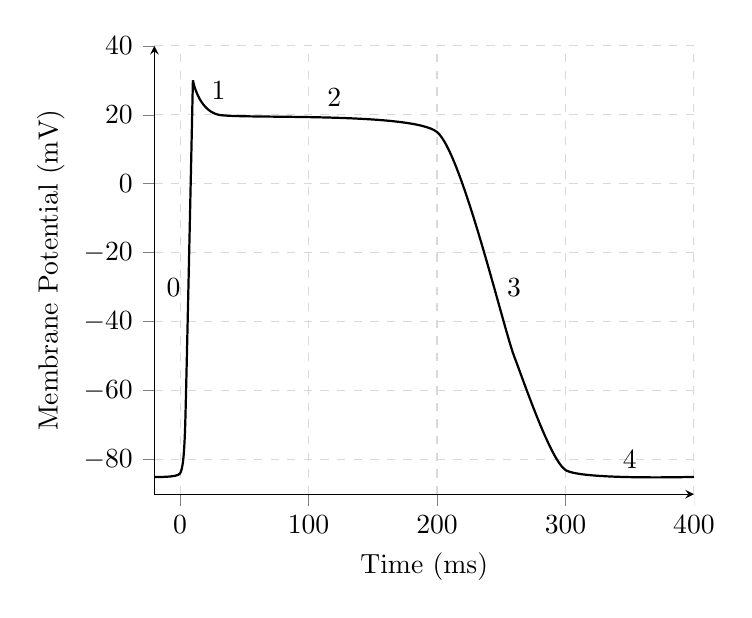
\begin{tikzpicture}

    \begin{axis}[
axis x line=bottom,
  axis y line=left,
	ymin = -90,
	ymax = 40,
	xmin = -20,
xmax = 400,
        grid = major,
        grid style={dashed, gray!30},
	 ylabel near ticks,
	xlabel near ticks,
        xlabel=Time (ms),
        ylabel=Membrane Potential (mV),
        tick align=outside,
        enlargelimits=false]

\draw[black, thick] plot[smooth,tension=0.3] coordinates { (axis cs: -20,-85) (axis cs: 0,-84) (axis cs: 4,-70) (axis cs: 10,30)};
\draw[black, thick] plot[smooth,tension=0.3] coordinates { (axis cs: 10,30) (axis cs: 30,20) (axis cs: 200,15) (axis cs: 260,-50) (axis cs: 300, -83) (axis cs: 400,-85)};


\node[black] at (axis cs: -5,-30){0};
\node[black] at (axis cs: 30,27){1};
\node[black] at (axis cs: 120,25){2};
\node[black] at (axis cs: 260,-30){3};
\node[black] at (axis cs: 350,-80){4};



\end{axis}

\end{tikzpicture} 
\end{document}